% !TeX program = pdflatex
% =============================================================
% Public Economics -- Lecture 6
% Inequality
% Based on: Leenders, W. "Microeconomics of Public Policy, Part III:
%           Inequality" (Sciences Po, MPA 2023-2024)
% Austrian institutional and empirical context added for WU Vienna.
% =============================================================
\documentclass[11pt,aspectratio=169]{beamer}

\usetheme{metropolis}
\usepackage[utf8]{inputenc}
\usepackage[T1]{fontenc}
\usepackage{lmodern}
\usepackage{booktabs}
\usepackage{array}
\usepackage{textcomp}
\usepackage{siunitx}
\usepackage{tikz}
\usepackage{pgfplots}
\pgfplotsset{compat=1.18}
\usepackage{pgf-pie}
\usetikzlibrary{positioning,arrows.meta,calc}

% ----------------------------------------------------------------
% Colors: WU Vienna blue as primary accent
% ----------------------------------------------------------------
\definecolor{wublue}{HTML}{003D7C}
\definecolor{wulight}{HTML}{4F8FC4}
\definecolor{wugray}{HTML}{5C6670}
\definecolor{wured}{HTML}{B0202E}
\definecolor{wugreen}{HTML}{4C8C6B}
\definecolor{wuyellow}{HTML}{D9A441}
\setbeamercolor{palette primary}{bg=wublue,fg=white}
\setbeamercolor{frametitle}{bg=wublue,fg=white}
\setbeamercolor{progress bar}{fg=wublue,bg=wulight!30}
\setbeamercolor{alerted text}{fg=wured}

\setbeamertemplate{frame footer}{Inequality}
\setbeamertemplate{footline}[frame number]

\title{Public Economics}
\subtitle{Lecture 6 \(\cdot\) Inequality}
\author{Shushanik Margaryan}
\institute{WU Vienna University of Economics and Business}
\date{Winter Term}

% Source note command for footnote-style citations on data slides
\newcommand{\srcnote}[1]{{\footnotesize\color{wugray}Source: #1}}

\begin{document}

% =============================================================
\begin{frame}
  \titlepage
\end{frame}

\begin{frame}{Today's Questions}
  \begin{itemize}
    \item What exactly do we mean by ``inequality,'' and why do economists --- and everyone else --- care about it?
    \item How do we measure inequality in income and in wealth, and what are the pitfalls of each approach?
    \item How much of a person's economic position is inherited from their parents, rather than earned?
  \end{itemize}
  \vspace{1em}
  \begin{block}{Based on}
    Leenders, W., \emph{Microeconomics of Public Policy, Part III: Inequality} (Sciences Po, 2023--2024).
  \end{block}
\end{frame}

% =============================================================
\begin{frame}{Outline}
  \tableofcontents
\end{frame}

% =============================================================
\section{6.1 What Is Inequality, and Why Do We Care?}

\begin{frame}{What Is Inequality?}
  \small
  Inequality refers to differences in resources between individuals or groups.
  \begin{itemize}
    \item \textbf{Type of resource}: income, wealth, consumption, ``opportunity.''
    \item \textbf{Type of group}: class, gender, region, generation, \ldots
    \item \textbf{Scope}: global, national, regional.
  \end{itemize}
  \vspace{0.3em}
  The World Inequality Lab tracks the most up-to-date research in the \emph{World Inequality Report} and at \href{https://wid.world}{wid.world}.
\end{frame}

\begin{frame}{Income Shares Around the World}
  \begin{center}
    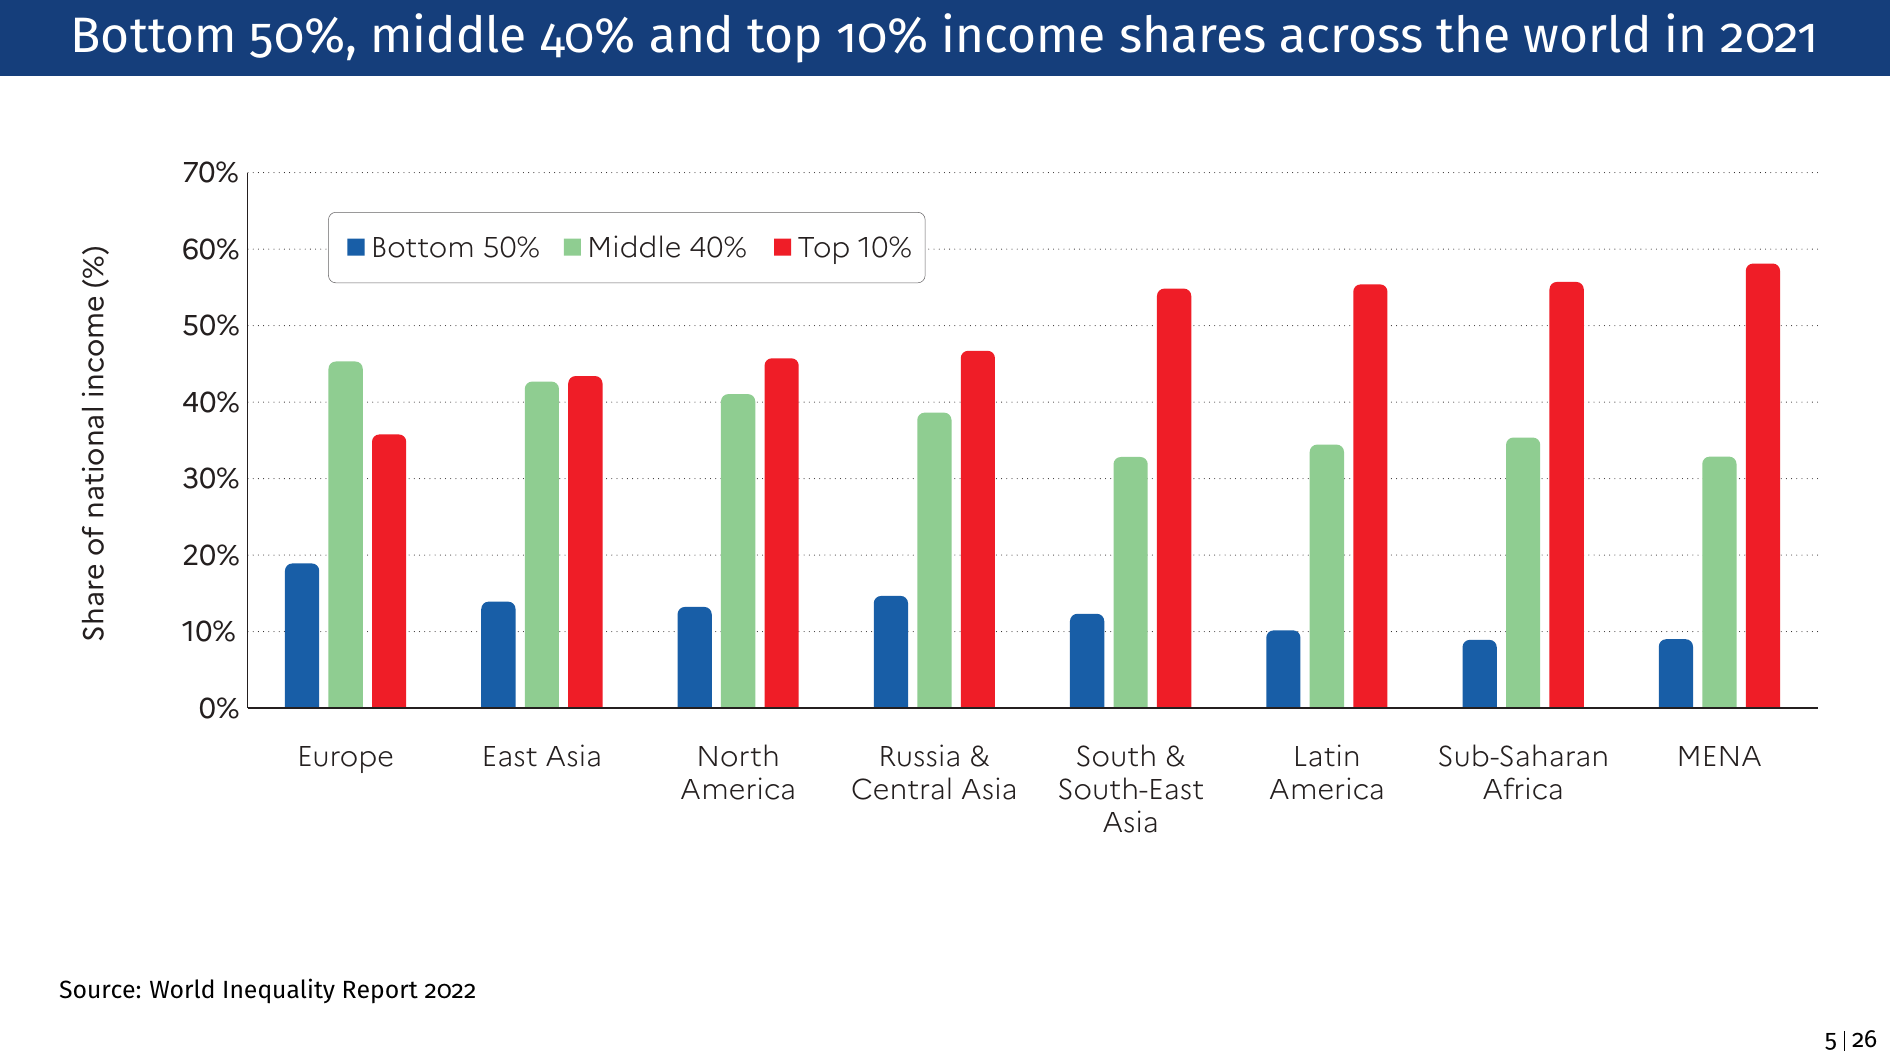
\includegraphics[height=5.3cm]{figures/world_income_shares_2021.png}
  \end{center}
  \centering
  \footnotesize
  In every world region, the top 10\% earns a far larger share of income than the bottom 50\%. Europe is the world's most equal region by this measure --- but still far from equal.\\
  \srcnote{World Inequality Report 2022.}
\end{frame}

\begin{frame}{Wealth Shares Around the World}
  \begin{center}
    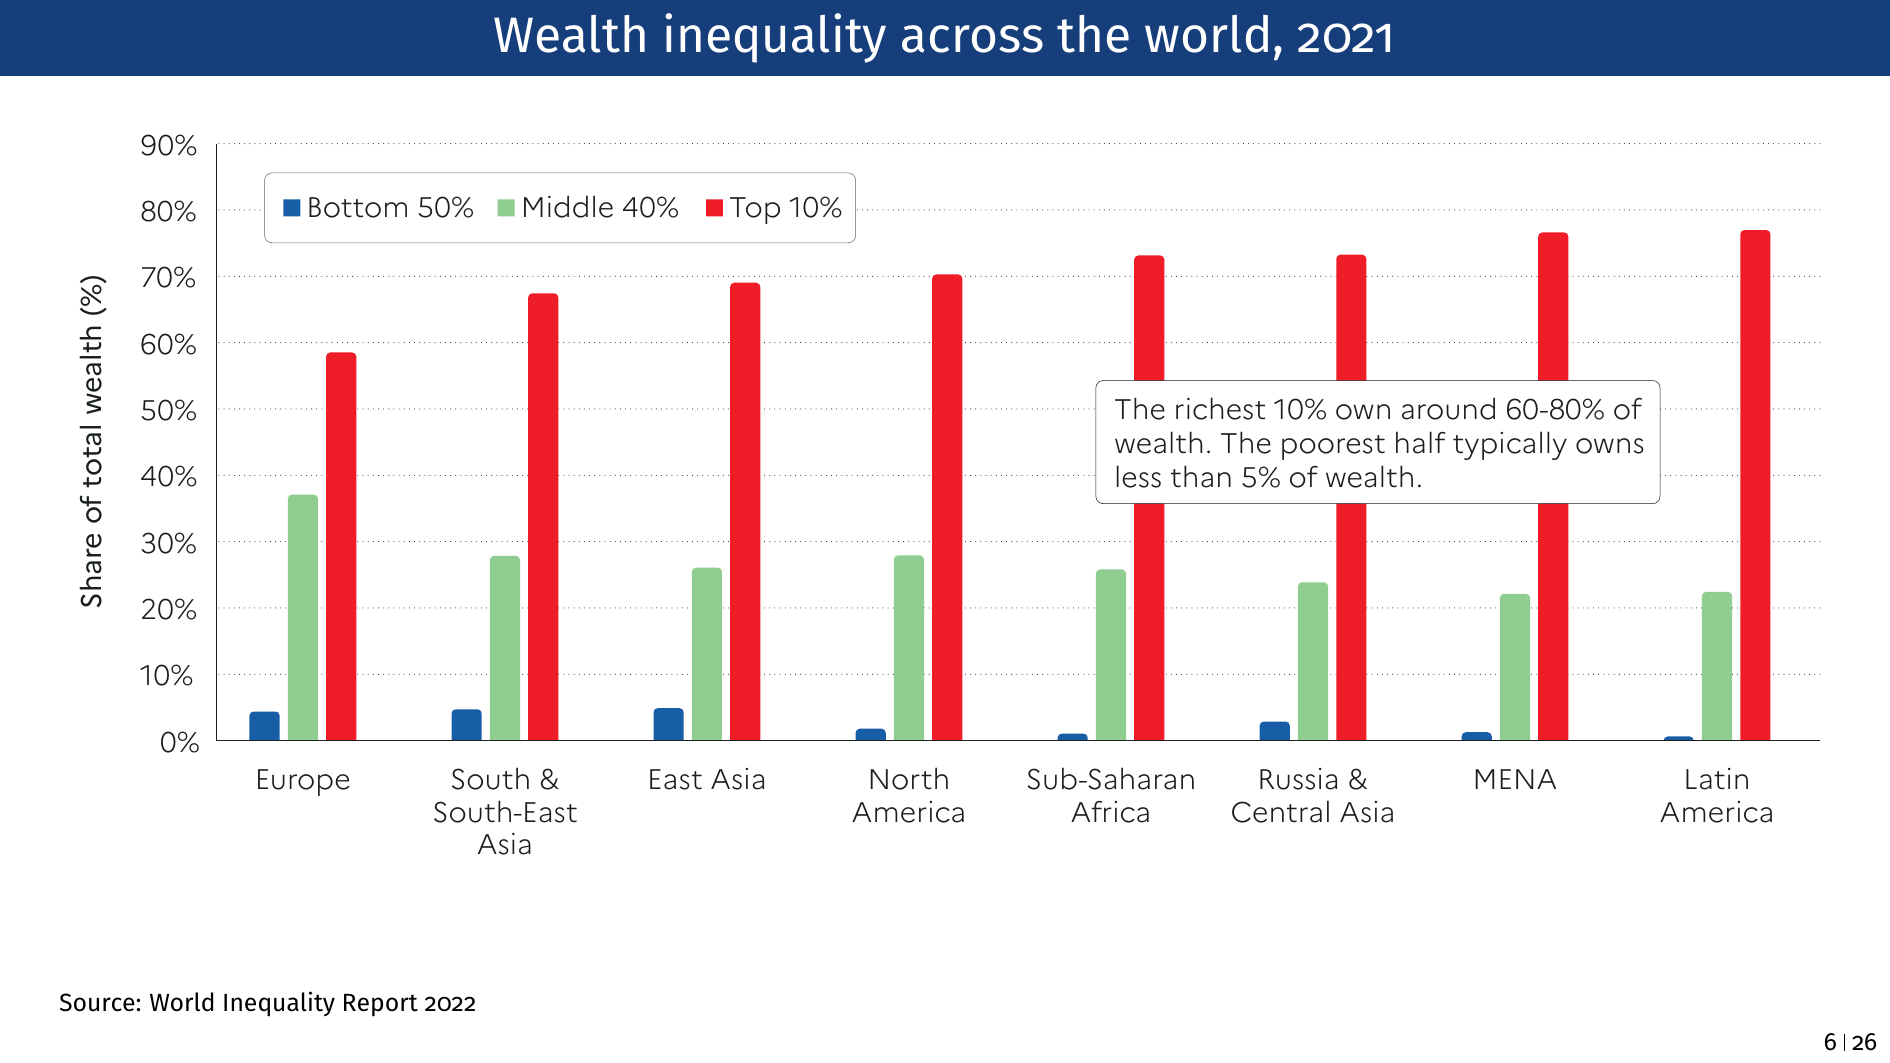
\includegraphics[height=5.3cm]{figures/world_wealth_shares_2021.png}
  \end{center}
  \centering
  \footnotesize
  The gap is wider still for wealth: the top 10\% typically owns 60--80\%, the bottom half less than 5\%, in every region shown.\\
  \srcnote{World Inequality Report 2022.}
\end{frame}

\begin{frame}{Why Do We Care?}
  \small
  \begin{itemize}
    \item \textbf{Eurobarometer}: 81\% of EU citizens agree that differences in income are too great.
    \item Biologists have documented an aversion to inequality among capuchin monkeys, apes, dogs, and birds (Brosnan \& de Waal, 2014) --- a sense of fairness may be evolutionarily old.
    \item Humans engage in joint production with others through families, firms, and the state. The fruits of that production need to be divided somehow --- which may explain why fairness concerns run so deep.
  \end{itemize}
  \vspace{0.3em}
  \centering
  \(\Rightarrow\) Emmanuel Saez's 2021 AEA Distinguished Lecture, \emph{``Public Economics and Inequality: Uncovering Our Social Nature.''}
\end{frame}

% =============================================================
\section{6.2 Measuring Inequality}

\begin{frame}{Income Shares and Summary Indices}
  \small
  \begin{itemize}
    \item Inequality is distinct from \textbf{poverty}: it concerns the \emph{relative} distribution of resources, not an absolute threshold.
    \item \textbf{Income shares} measure how much of total income accrues to a given group --- the bottom 50\%, the top 10\%, the top 0.01\%.
    \item \textbf{Indices} compress the whole distribution into a single number: the Gini coefficient, the Atkinson index, the Theil index.
  \end{itemize}
  \vspace{0.3em}
  \begin{alertblock}{The cost of simplicity}
    A single number is easy to compare across countries and years --- but it collapses a complex, multidimensional concept, and (changes in) it are often hard for non-experts to interpret (Piketty, \emph{Capital in the 21st Century}, pp.\ 266--267).
  \end{alertblock}
\end{frame}

\begin{frame}{The Gini Coefficient}
  \begin{columns}[T]
    \begin{column}{0.55\textwidth}
      \begin{center}
        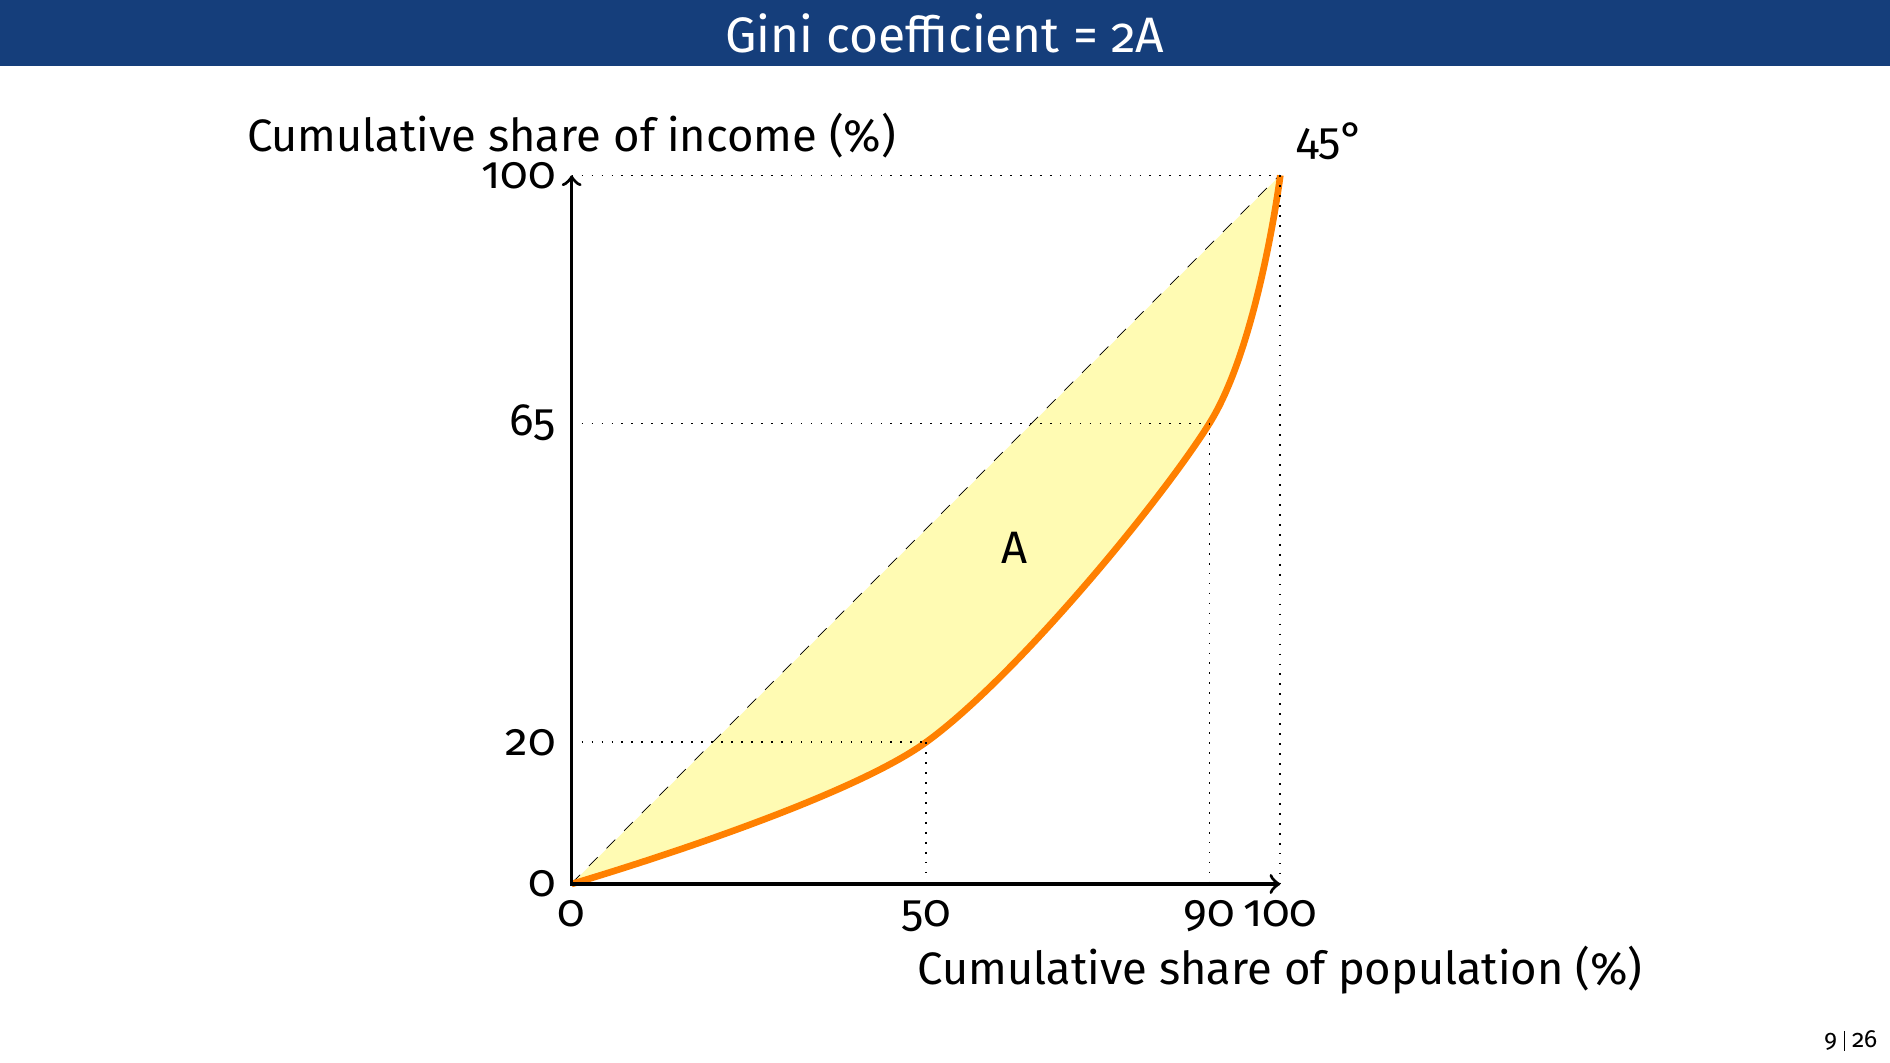
\includegraphics[width=\textwidth]{figures/gini_lorenz_diagram.png}
      \end{center}
    \end{column}
    \begin{column}{0.45\textwidth}
      \small
      \begin{itemize}
        \item Plot the \textbf{Lorenz curve}: the cumulative share of income earned by the bottom $x$\% of the population.
        \item Perfect equality is the 45\textdegree\ line; the further the Lorenz curve sags below it, the more unequal the distribution.
        \item \textbf{Gini} $= 2A$, where $A$ is the area between the two curves --- ranges from 0 (perfect equality) to 1 (perfect inequality).
      \end{itemize}
    \end{column}
  \end{columns}
\end{frame}

\begin{frame}{Data on Inequality: Surveys vs.\ Tax Records}
  \footnotesize
  \begin{itemize}
    \item \textbf{Household surveys} are the traditional source --- but the sample is often too small to say much about the top, incomes/wealth above a threshold are often top-coded, and very few surveys existed before the 1950s.
    \item \textbf{Tax data} (Pareto, Kuznets, Piketty--Saez tradition) reach further into the top of the distribution, but are distorted by tax evasion, differ across countries' tax laws, and don't map cleanly onto macroeconomic income concepts (GDP, national income).
  \end{itemize}
  \vspace{0.3em}
  \begin{alertblock}{Distributional national accounts (DINA)}
    A newer approach reconciles survey and tax data with macroeconomic aggregates, using a consistent, comprehensive income definition --- measured both before and after taxes and transfers. Austria has its own DINA series (Jestl \& List, 2020, 2004--2016) --- recall Lecture 1.
  \end{alertblock}
\end{frame}

% =============================================================
\section{6.3 Income Inequality}

\begin{frame}{What Is Income?}
  \small
  \textbf{National income} = domestic output, net of capital depreciation, plus net foreign income --- made up of \textbf{labor income} ($\approx$70--75\%) and \textbf{capital income} ($\approx$25--30\%).
  \vspace{0.3em}
  \begin{columns}[T]
    \begin{column}{0.5\textwidth}
      \textbf{Labor income} (wages, pensions, fringe benefits) inequality comes from:
      \begin{itemize}
        \item Education and skills
        \item Labor-market institutions (unions, minimum wages)
        \item Work effort
        \item Social norms and discrimination
      \end{itemize}
    \end{column}
    \begin{column}{0.5\textwidth}
      \textbf{Capital income} (profits, interest, rent) inequality comes from:
      \begin{itemize}
        \item Wealth inequality itself
        \item Inequality in \emph{rates of return} on that wealth
      \end{itemize}
    \end{column}
  \end{columns}
\end{frame}

\begin{frame}{Pre-Tax and Post-Tax Inequality}
  \small
  Governments redistribute income through taxation (Lecture 4) and government spending:
  \begin{itemize}
    \item \textbf{Cash transfers}: pensions, unemployment benefits, social assistance.
    \item \textbf{In-kind transfers}: goods/services provided free or below cost (healthcare, education).
    \item \textbf{Collective expenditure}: non-rival spending consumed passively by everyone (defense, infrastructure).
  \end{itemize}
  \vspace{0.3em}
  \centering
  Government spending runs 30--50\% of GDP across rich democracies --- so the gap between \emph{pre-tax} and \emph{post-tax} inequality can be large.
\end{frame}

\begin{frame}{Predistribution, Not Just Redistribution}
  \footnotesize
  \begin{center}
  \begin{tabular}{@{}lcccc@{}}
    \toprule
     & \multicolumn{2}{c}{\textbf{Pre-tax}} & \multicolumn{2}{c}{\textbf{Post-tax}} \\
    \textbf{Top 1\% income share} & 1980 & 2017 & 1980 & 2017 \\
    \midrule
    United States & 11\% & 21\% & 9\% & 16\% \\
    Europe & 8\% & 11\% & 7\% & 9\% \\
    \bottomrule
  \end{tabular}
  \end{center}
  \vspace{0.3em}
  \begin{itemize}
    \item Blanchet, Chancel \& Gethin (2022) construct distributional national accounts for 26 European countries, 1980--2017.
    \item Europe redistributes a \emph{larger} fraction of output overall --- but US redistribution is more targeted at the bottom 50\%.
    \item \textbf{Predistribution} (a more equal distribution \emph{before} taxes and transfers) --- not redistribution --- is the main reason Europe ends up more equal than the US.
  \end{itemize}
  \srcnote{Blanchet, Chancel \& Gethin, ``Why Is Europe More Equal than the United States?'' \emph{AEJ: Applied Economics} 14(4), 2022.}
\end{frame}

\begin{frame}{Austria in the OECD Income Distribution}
  \footnotesize
  \begin{center}
  \begin{tabular}{@{}lcccccc@{}}
    \toprule
    & \textbf{Bottom} & \textbf{2nd} & \textbf{3rd} & \textbf{4th} & \textbf{Highest} & \textbf{Top 10\%} \\
    \midrule
    Sweden & 10.7\% & 14.4\% & 17.6\% & 21.5\% & 35.7\% & 10.9\% \\
    \textbf{Austria} & \textbf{8.4\%} & \textbf{12.4\%} & \textbf{16.8\%} & \textbf{22.3\%} & \textbf{40.1\%} & \textbf{13.6\%} \\
    France & 9.4\% & 12.9\% & 16.3\% & 21.0\% & 40.4\% & 15.2\% \\
    United States & 3.3\% & 8.5\% & 14.6\% & 23.4\% & 50.2\% & 21.3\% \\
    OECD average & 8.5\% & 12.2\% & 16.0\% & 21.1\% & 42.2\% & 16.7\% \\
    \bottomrule
  \end{tabular}
  \end{center}
  \vspace{0.3em}
  \centering
  Austria sits close to the Nordic end of the distribution --- more equal than the OECD average, and far more equal than the US.\\
  \srcnote{Gruber, \emph{Public Finance and Public Policy}, \S17.1, income-quintile shares by country.}
\end{frame}

\begin{frame}{Austria's Gini Coefficient: Stable, Then Rising}
  \small
  \begin{itemize}
    \item Austria's most recent income Gini coefficient (equivalised disposable household income) is \textbf{28.4} (EU-SILC 2024 release, income year 2023) --- just below the EU-27 average of \textbf{29.4}.
    \item Halla \& Weber (2024) find Austria's income inequality was \textbf{broadly stable from 2004--2019}, despite major labor-market shifts over that period: rising female labor-force participation, educational upgrading, and growth in part-time and cross-border work.
    \item More recently, Statistik Austria reports the Gini \textbf{rose for three consecutive years} through 2024 --- the highest level in the EU-SILC series to date.
  \end{itemize}
  \vspace{0.3em}
  \centering
  A low, stable headline number can still mask a recent turning point --- always check whether ``stable'' inequality is still stable in the latest data.\\
  \srcnote{Eurostat, EU-SILC (\texttt{ilc\_di12}); Halla \& Weber, ``Persistent Low Inequality Despite Compositional Shifts in Austria,'' \emph{Fiscal Studies} 45(3), 2024; Statistik Austria, Einkommen und Armut 2024.}
\end{frame}

\begin{frame}{Real-Time Inequality}
  \small
  \begin{itemize}
    \item The World Inequality Lab's \href{https://realtimeinequality.org}{realtimeinequality.org} combines national accounts, tax, and survey \emph{micro}data to estimate income growth by group, updated quarterly --- rather than waiting years for the next official release.
    \item Recent readings consistently show income growth \textbf{rising with income rank}: the top 0.01\% grows fastest, the bottom 50\% slowest.
  \end{itemize}
  \vspace{0.3em}
  \centering
  \alert{Real-time measurement is itself a research frontier --- most official inequality statistics still arrive with a multi-year lag.}\\
  \srcnote{Blanchet, Saez \& Zucman, ``Real-Time Inequality,'' working paper, 2022.}
\end{frame}

% =============================================================
\section{6.4 Wealth Inequality}

\begin{frame}{What Is Wealth?}
  \small
  \textbf{Wealth} = the sum of all assets minus the sum of all liabilities.
  \begin{itemize}
    \item An \textbf{asset} is a store of value representing expected future economic benefits: real estate, equity, bonds, deposits.
    \item A \textbf{liability} is the converse: mortgages, student loans, consumer debt.
  \end{itemize}
  \vspace{0.3em}
  \centering
  Wealth can be owned by private individuals \emph{or} by the government --- which is why \textbf{public} wealth matters for inequality too, not just private wealth.
\end{frame}

\begin{frame}{The Rise of Private Wealth, the Fall of Public Wealth}
  \begin{columns}[T]
    \begin{column}{0.52\textwidth}
      \begin{center}
        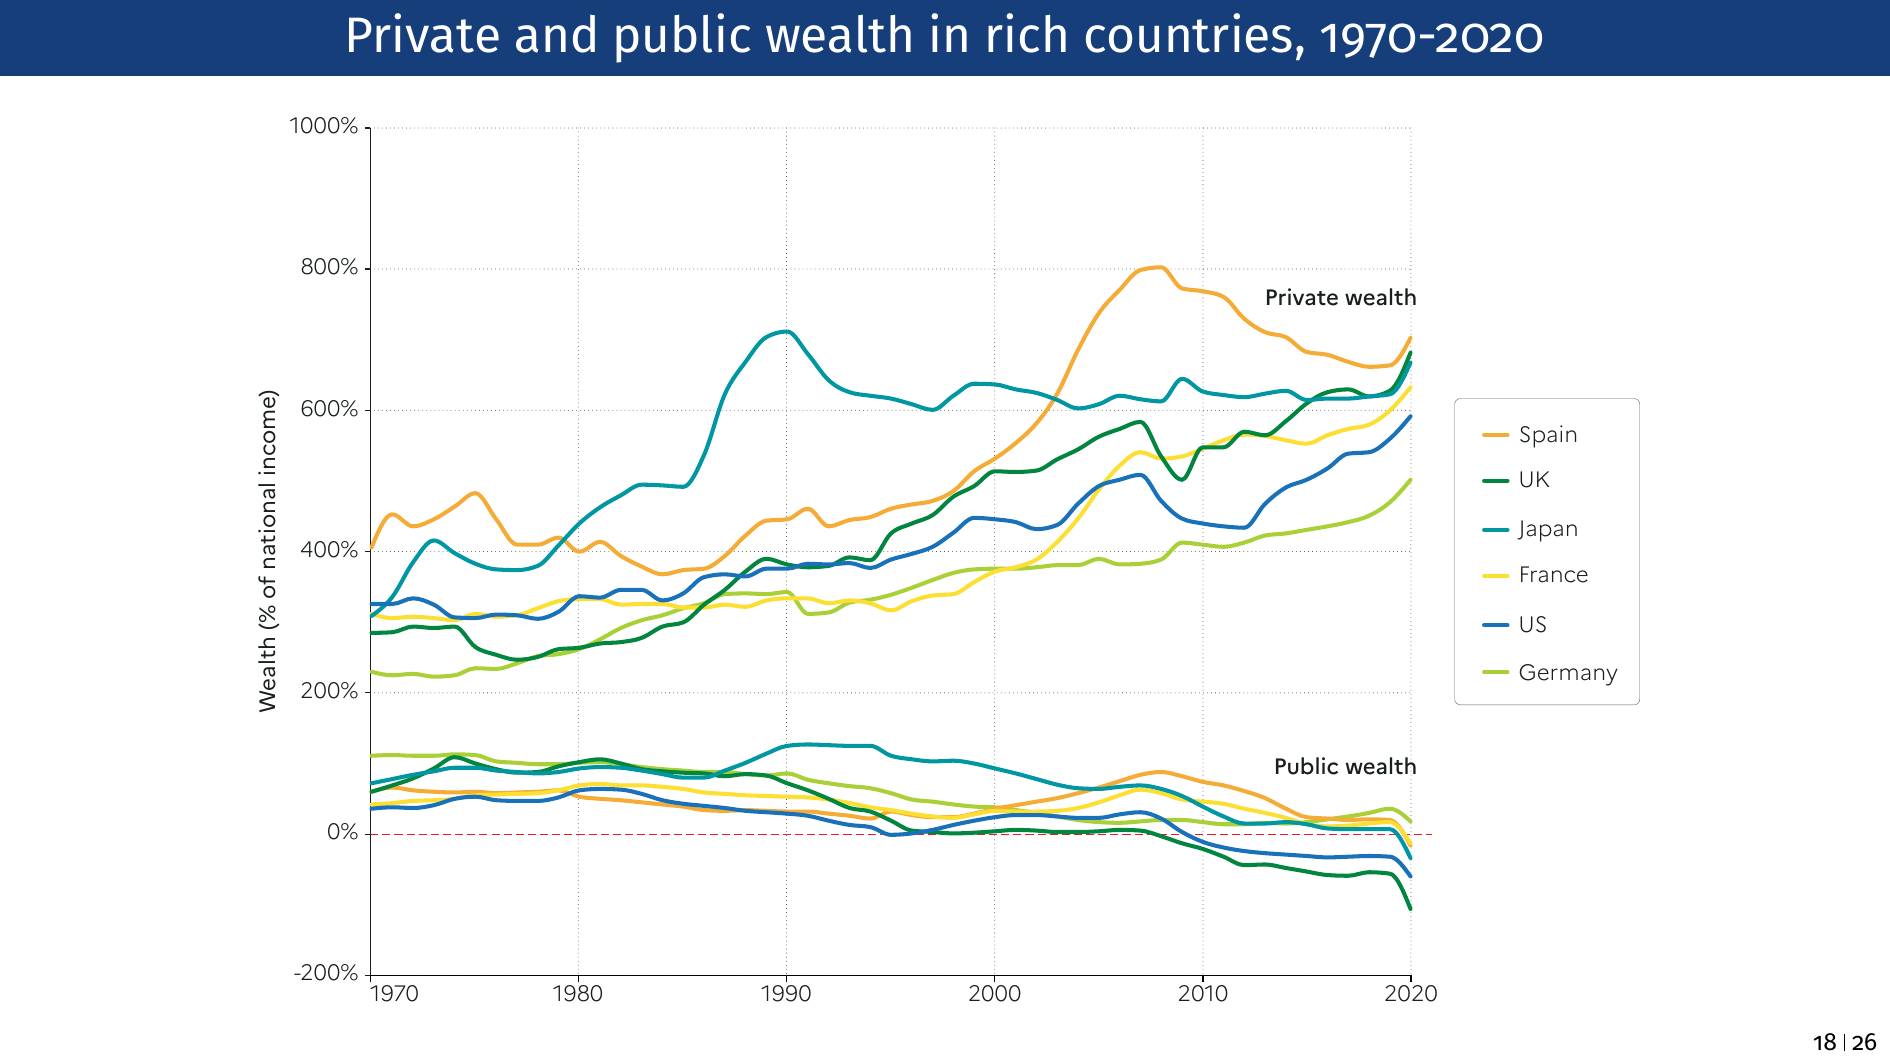
\includegraphics[width=\textwidth]{figures/private_public_wealth_1970_2020.png}
      \end{center}
    \end{column}
    \begin{column}{0.48\textwidth}
      \scriptsize
      \begin{itemize}
        \setlength{\itemsep}{2pt}
        \item Across rich countries since 1970, \textbf{private} wealth has risen relative to national income --- while \textbf{public} wealth stagnated or turned negative.
        \item Austria's own version: abolishing the \textbf{wealth tax} (1994) and letting the \textbf{inheritance tax} lapse (2008) (Lecture 4) removed two tools governments elsewhere use to tax accumulated wealth.
        \item A government that owns less has less room to cushion shocks or redistribute, without new borrowing or taxation.
      \end{itemize}
    \end{column}
  \end{columns}
  \srcnote{Blanchet \& Martínez-Toledano, \emph{Journal of Monetary Economics} 133, 2023.}
\end{frame}

\begin{frame}{How Do We Measure Wealth?}
  \footnotesize
  \begin{itemize}
    \item The ideal source would be a well-enforced, comprehensive \textbf{wealth tax} --- but few countries levy one (Austria included, since 1994).
    \item In its absence, \textbf{surveys} like the ECB's \emph{Household Finance and Consumption Survey} (HFCS) --- which includes Austria, run by the OeNB --- collect wealth data directly.
    \item \textbf{Inheritance tax records} offer an old alternative: treat estates as a (non-random) sample of wealth and correct for the selection.
    \item Capital income can be \textbf{``capitalised''}: $Y_k = rK \Rightarrow K = Y_k/r$, inferring wealth from the capital income it generates.
    \item \textbf{Rich lists} (Forbes 400, Bloomberg Billionaires Index) compile journalist estimates of the very top.
  \end{itemize}
\end{frame}

\begin{frame}{Austria's Wealth Concentration: A Measurement Case Study}
  \small
  \begin{itemize}
    \item Austria's HFCS 2021 wave (OeNB) puts the net-wealth Gini coefficient at \(\approx\)\textbf{0.70} --- and the top 10\% of households hold \(\approx\)\textbf{51\%} of net wealth, among the highest concentrations in the euro area.
    \item The raw survey data put the top 1\% share at \(\approx\)\textbf{25\%} --- but HFCS-style surveys systematically \textbf{undersample the ultra-wealthy} (too few billionaires answer a household survey).
    \item Correcting for this with rich-list-calibrated methods, OeNB researchers Fessler \& Schürz estimate Austria's true top 1\% share is closer to \(\approx\)\textbf{43\%}.
  \end{itemize}
  \vspace{0.3em}
  \centering
  This is the measurement problem from two slides ago, playing out in real data: the ``right'' answer for Austria's wealth concentration nearly doubles once you correct for who a household survey misses.\\
  \srcnote{OeNB, Eurosystem HFCS 2021 -- First Results for Austria (2023); Fessler \& Schürz, ``The Size and Distribution of Augmented Wealth,'' \emph{Journal of Pension Economics \& Finance}, 2026.}
\end{frame}

\begin{frame}{What Drives Wealth Inequality?}
  \small
  Wealth owned by individual $i$ in period $t+1$ depends on wealth in period $t$, the saving rate, and the rate of return:
  \[
    W^i_{t+1} = (1+r^i_t)\left(W^i_t + s^i_t \, Y^i_t\right)
  \]
  \vspace{0.2em}
  Differences in wealth can therefore come from:
  \begin{enumerate}
    \item Pre-existing differences in wealth
    \item Labor income inequality
    \item Differential saving rates
    \item Differential rates of return $r^i_t$
  \end{enumerate}
\end{frame}

\begin{frame}{Wealth Concentration: Europe vs.\ the US}
  \small
  \begin{center}
  \begin{tabular}{@{}lcc@{}}
    \toprule
    \textbf{Top 1\% wealth share} & \textbf{1970} & \textbf{2020} \\
    \midrule
    United States & 27\% & 35\% \\
    Europe & 24\% & 24\% \\
    \bottomrule
  \end{tabular}
  \end{center}
  \vspace{0.3em}
  \begin{itemize}
    \item Blanchet \& Martínez-Toledano (2023) construct distributional wealth accounts for 31 European countries, 1970--2020.
    \item Wealth concentration has risen in both Europe and the US recently --- but far more in the US.
    \item Two explanations: European house prices rose by \emph{more} (which spreads gains toward middle-wealth homeowners), and European labor-income inequality rose by \emph{less}.
  \end{itemize}
\end{frame}

% =============================================================
\section{6.5 Intergenerational Mobility}

\begin{frame}{How Do We Measure Mobility?}
  \small
  How much does parental income shape a child's own economic success --- a common (if imperfect) proxy for ``inequality of opportunity''?
  \begin{itemize}
    \item \textbf{Intergenerational elasticity of income}: by how much does a child's income rise if their parents' income rises by 1\%?
    \item \textbf{Rank-rank correlation}: the correlation between a parent's income rank and their child's.
    \item \textbf{Absolute mobility}: the expected income rank of a child born to parents at percentile $p$.
  \end{itemize}
\end{frame}

\begin{frame}{The US Is Less Mobile than Denmark}
  \begin{center}
    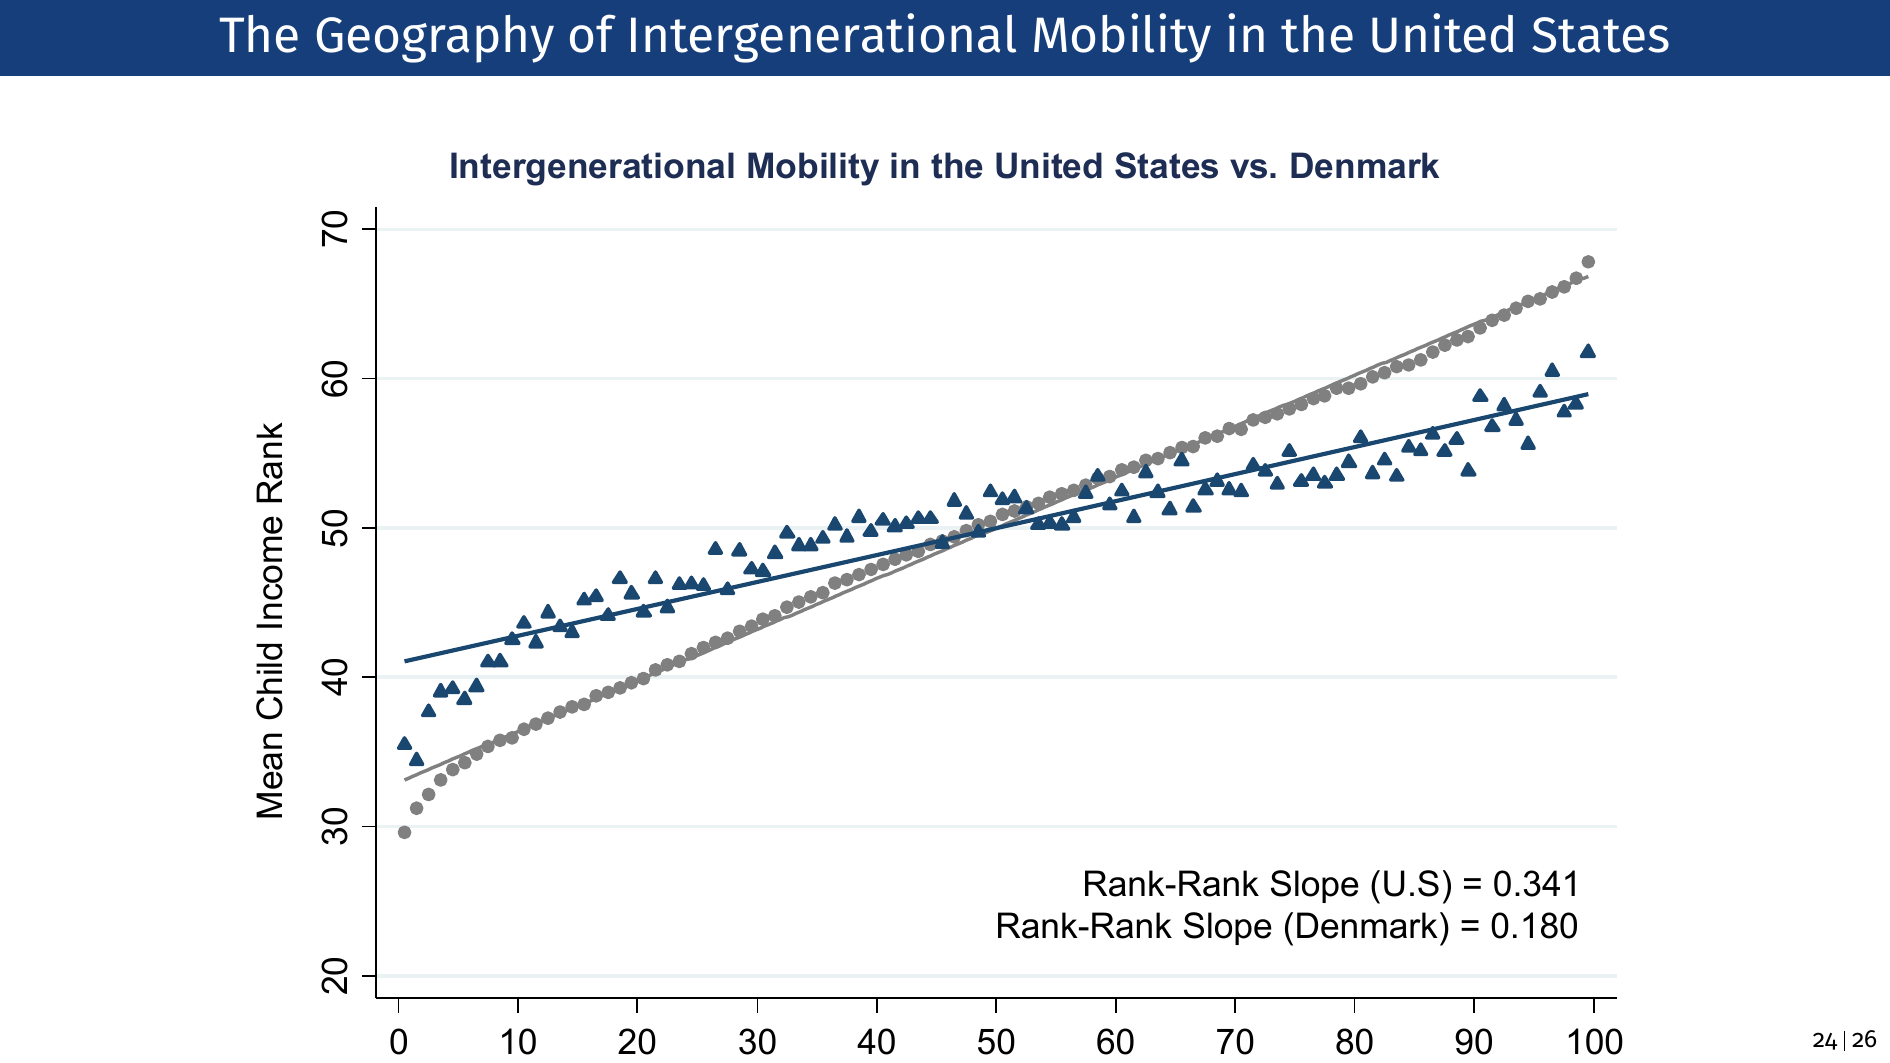
\includegraphics[height=5.4cm]{figures/mobility_us_denmark_scatter.png}
  \end{center}
  \centering
  \footnotesize
  A flatter slope means a child's income is less tied to their parents' --- \textbf{more} mobility. The US rank-rank slope (0.341) is nearly double Denmark's (0.180).\\
  \srcnote{Chetty, Hendren, Kline \& Saez, ``Where Is the Land of Opportunity?'' \emph{QJE} 129(4), 2014.}
\end{frame}

\begin{frame}{Mobility Varies Enormously \emph{Within} Countries Too}
  \begin{columns}[T]
    \begin{column}{0.52\textwidth}
      \begin{center}
        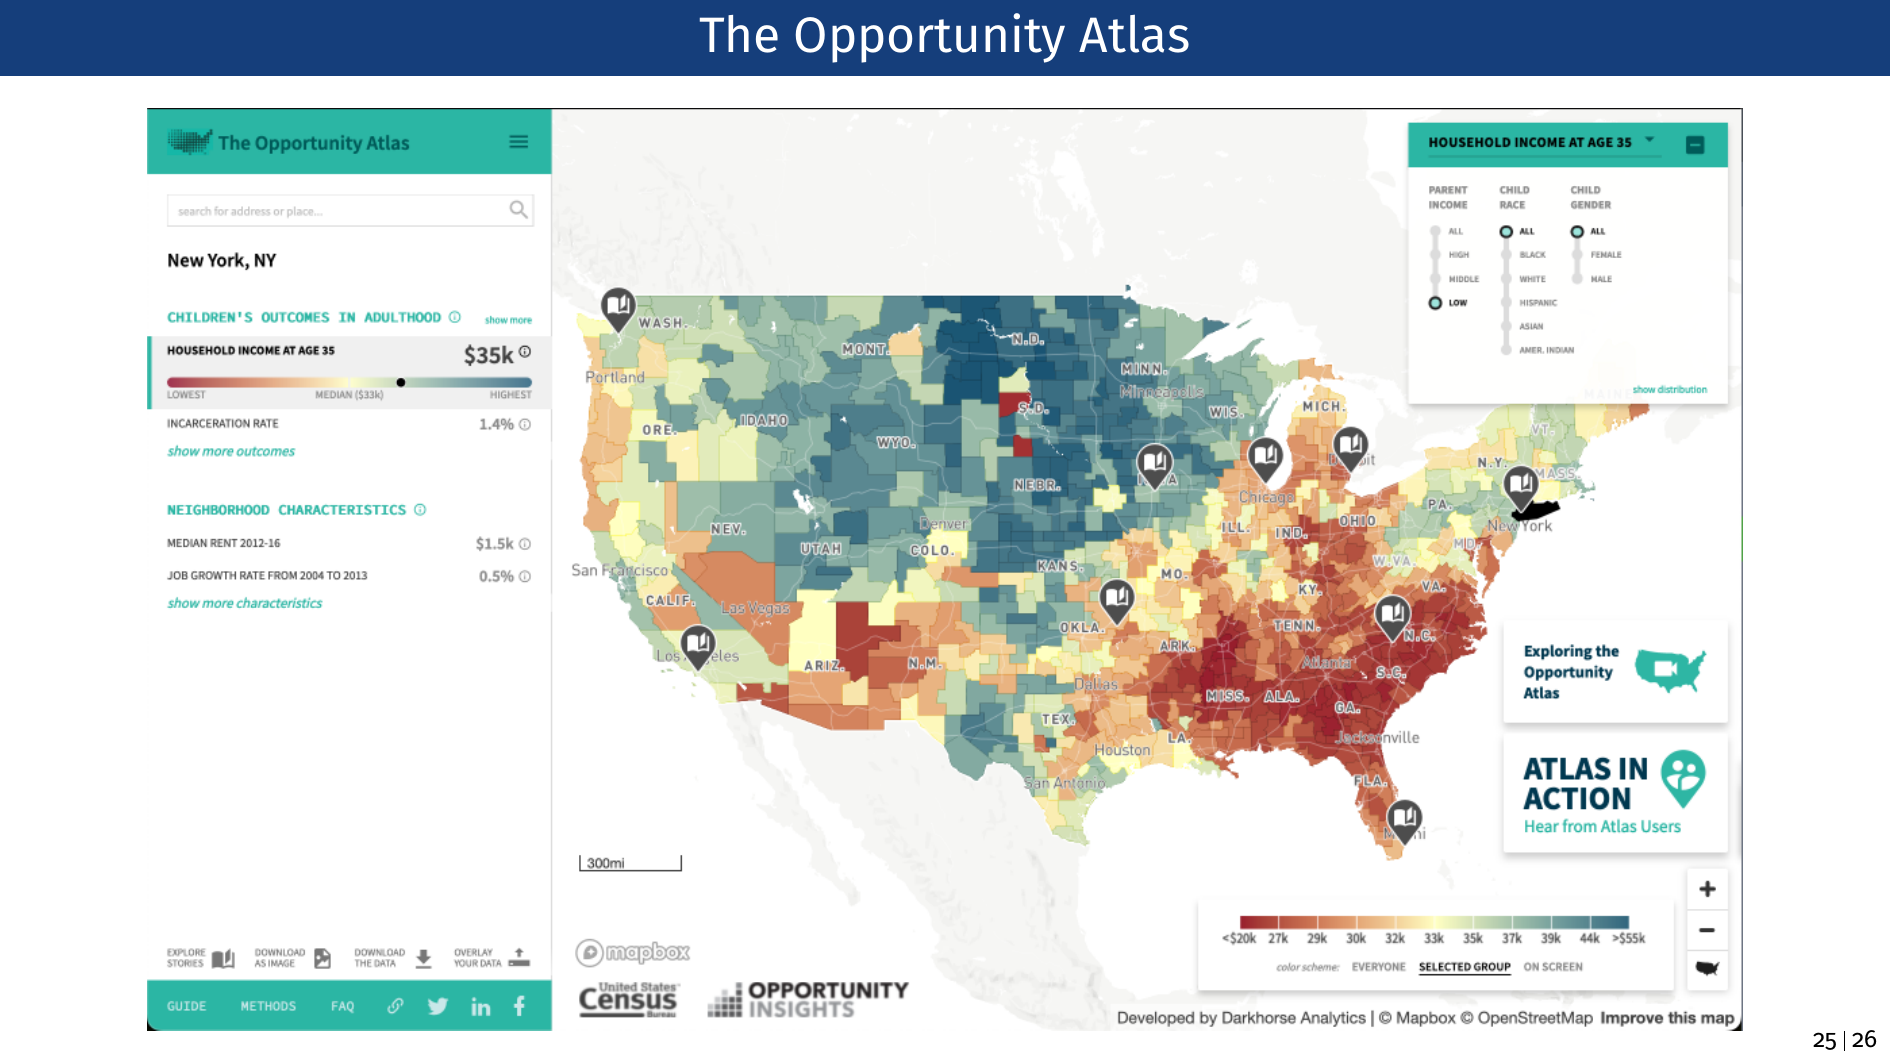
\includegraphics[width=\textwidth]{figures/opportunity_atlas_screenshot.png}
      \end{center}
    \end{column}
    \begin{column}{0.48\textwidth}
      \scriptsize
      \begin{itemize}
        \setlength{\itemsep}{2pt}
        \item Chetty et al.\ (2014) map absolute upward mobility across every US commuting zone using tax records --- the interactive \textbf{Opportunity Atlas} lets users explore outcomes down to the neighborhood level.
        \item Mobility is systematically \textbf{lower} in the US South, higher in the Midwest and Northeast --- differences as large as the US-vs-Denmark gap, \emph{within a single country}.
      \end{itemize}
    \end{column}
  \end{columns}
  \vspace{0.2em}
  \centering
  \footnotesize
  \alert{National averages can hide as much as they reveal --- the same is likely true of mobility across Austria's own regions, even without an Opportunity-Atlas-style tool to show it.}\\
  \srcnote{Chetty, Hendren, Kline \& Saez (2014); opportunityinsights.org.}
\end{frame}

\begin{frame}{Austria's Own Mobility Paradox}
  \footnotesize
  \begin{itemize}
    \item Despite its comparatively low income inequality, the OECD finds Austria's \textbf{intergenerational mobility lags behind many other OECD countries} --- a father's earnings are an unusually strong predictor of his children's adult earnings.
    \item Schnetzer \& Altzinger (2013) estimate an intergenerational income \emph{correlation} of \(\approx\)\textbf{0.13} for Austria (EU-SILC data) --- European mid-range: more mobile than Southern Europe, less than the Nordics. (A correlation, not the elasticity used in the US/Denmark slopes above --- not directly comparable.)
  \end{itemize}
  \vspace{0.2em}
  \begin{alertblock}{A gap worth naming}
    The OECD's cross-country ``generations to reach the average income'' measure (previous slides) has no published Austria-specific figure in the underlying table --- even rich-country statistical infrastructure has real gaps.
  \end{alertblock}
  \srcnote{OECD, \emph{Promoting Social Mobility in Austria} (2020); Schnetzer \& Altzinger, \emph{Momentum Quarterly} 2(3), 2013.}
\end{frame}

% =============================================================
\section{Conclusion}

\begin{frame}{Highlights}
  \small
  \begin{itemize}
    \item Inequality is multidimensional --- income vs.\ wealth, pre-tax vs.\ post-tax, national vs.\ within-country --- and no single index captures all of it.
    \item Europe is more equal than the US mainly through \textbf{predistribution} (a more equal starting distribution), not just heavier redistribution.
    \item Wealth is far more concentrated than income everywhere, and driven by a compounding process: existing wealth, saving rates, and rates of return all interact.
    \item Austria has neither a wealth tax nor an inheritance tax --- an unusually light institutional touch on accumulated wealth, even by European standards.
    \item Intergenerational mobility differs sharply across countries (US vs.\ Denmark) --- and just as sharply \emph{within} them.
  \end{itemize}
\end{frame}

\begin{frame}{Discussion Questions for Next Time}
  \small
  \begin{enumerate}
    \item If predistribution matters more than redistribution for Europe's relative equality, what pre-tax institutions (labor-market, educational) should get more attention than they currently do?
    \item Austria abolished its wealth and inheritance taxes decades ago. Given what drives wealth inequality (the formula on the wealth-inequality slide), what would reintroducing one actually change?
    \item Rank-rank mobility in the US is roughly double that of Denmark. What Danish institutions --- education, labor market, welfare state --- are the most plausible explanations?
    \item Should Austria build its own ``Opportunity Atlas''? What would it take, data-wise, and what might it reveal about mobility across Austria's own Bundesländer?
  \end{enumerate}
\end{frame}

\begin{frame}{Sources}
  \tiny
  \begin{columns}[T]
    \begin{column}{0.34\textwidth}
      \begin{itemize}
      \setlength{\itemsep}{3pt}
        \item Leenders, W., \emph{Microeconomics of Public Policy, Part III: Inequality}, lecture slides, Sciences Po (MPA 2023--2024).
        \item Chancel, Piketty, Saez \& Zucman, \emph{World Inequality Report 2022}, Harvard University Press.
        \item Blanchet, Chancel \& Gethin, ``Why Is Europe More Equal than the United States?'' \emph{AEJ: Applied Economics} 14(4), 2022.
        \item Blanchet \& Martínez-Toledano, ``Wealth Inequality Dynamics in Europe and the United States,'' \emph{Journal of Monetary Economics} 133, 2023.
        \item Blanchet, Saez \& Zucman, ``Real-Time Inequality,'' working paper, 2022.
      \end{itemize}
    \end{column}
    \begin{column}{0.33\textwidth}
      \begin{itemize}
      \setlength{\itemsep}{3pt}
        \item Halla \& Weber, ``Persistent Low Inequality Despite Compositional Shifts in Austria,'' \emph{Fiscal Studies} 45(3), 2024.
        \item Eurostat, EU-SILC (\texttt{ilc\_di12}); Statistik Austria, Einkommen und Armut 2024.
        \item OeNB, Eurosystem HFCS 2021 --- First Results for Austria (2023).
        \item Fessler \& Schürz, ``The Size and Distribution of Augmented Wealth,'' \emph{Journal of Pension Economics \& Finance}, 2026.
        \item Jestl \& List (2020), Austrian Distributional National Accounts, 2004--2016 --- Lecture 1.
      \end{itemize}
    \end{column}
    \begin{column}{0.33\textwidth}
      \begin{itemize}
      \setlength{\itemsep}{3pt}
        \item Chetty, Hendren, Kline \& Saez, ``Where Is the Land of Opportunity? The Geography of Intergenerational Mobility in the United States,'' \emph{QJE} 129(4), 2014.
        \item OECD, \emph{Promoting Social Mobility in Austria}, 2020.
        \item Schnetzer \& Altzinger, \emph{Momentum Quarterly} 2(3), 2013.
        \item Brosnan \& de Waal, ``Evolution of Responses to (Un)fairness,'' \emph{Science} 346, 2014.
        \item Piketty, T., \emph{Capital in the 21st Century}, Harvard University Press, 2014.
        \item Gruber, J. \emph{Public Finance and Public Policy}, \S17.1.
      \end{itemize}
    \end{column}
  \end{columns}
\end{frame}

\begin{frame}[standout]
  Thank you!\\
  \vspace{0.5em}
  \small Questions and discussion
\end{frame}

\end{document}
